\chapter{Pi power}
\minitoc
\notesurl{intro3}

So far you've used your Pi and the lab PCs separately, and hopefully you've come to understand that they are both essentially the same kind of machine; they both run variations of the same operating system, and the principles you learn using one for the most part apply to the other. In the case of the Pi, you have complete control of the device as a superuser, so can do absolutely what you like to it; in the case of the lab machines you have access to much more powerful hardware, but more restricted access to the filestore and operating system for reasons of security and privacy.

Today, we'll be getting your Pi and a desktop PC to communicate with one another, to reinforce the similarities between these setups, and to expose you to some of the principles of networking and remote access.

\section{The LXDE graphical environment}

Connect your Pi up to the monitor, keyboard, mouse, network and power supply as before, and log in (remembering this time to use whatever password you set on the Pi rather than your University password, and the username `pi'). At the console, type:

\begin{ttoutenv}
\$ startx
\end{ttoutenv}

to start up X Windows and the Pi's default window manager, LXDE, which appear moments later looking like the screenshot in Figure \ref{figure:lxde-desktop}.

LXDE (the `Lightweight X11 Desktop Environment') is designed to be a lean, fast desktop environment, which makes it ideally suited for the Pi's modest CPU. Although rather less rich in features and `eyecandy' than GNOME, LXDE is a fully functioning environment that has all the features you will need for operating and programming the Pi.


\begin{linux}{LXDE isn't a window manager either}
Rather like GNOME, LXDE is a technically a collection of desktop tools rather than a window manager as such. LXDE uses the \wikipedia{Openbox}{openbox} window manager, and \wikipedia{GTK+}{GTK+}, which was developed as part of the \wikipedia{GIMP}{GIMP} project to draw the buttons, sliders and other graphical controls. LXDE is the default graphical environment for several `lean' or `low power' Linux distributions such as \wikipedia{Knoppix}{Knoppix}, \wikipedia{Lubuntu}{Lubuntu} and of course the Pi's operating system, \wikipedia{Raspbian}{Raspbian}.
\end{linux}

Up at the top of the screen you will see LXDE's `panel'. On the left of the panel (\protect\circled{1} in the figure) are controls that give you access to various applications, tools and system preferences. On the panel's right (marked \protect\circled{2}) are a CPU meter and a clock. On the desktop itself is a shortcut to the Wastebasket, which is similar to the Recycle Bin on Windows and the Trash on OS X.

Spend a few minutes exploring the GUI. You may find that you're double-clicking on things that only need a single click, and vice versa, and may find that things aren't quite where you expect them to be---but rather than dismissing LXDE as being crude, embrace the differences; you may well find that you come to prefer its `no frills' approach to window management over that of richer, heavier-weight environments such as GNOME. LXDE and other slimmed-down graphical environments consume considerably fewer CPU cycles and hence less power than their richer counterparts, and while this isn't an issue when you're running on a mains-powered desktop machine with a reasonably beefy graphics card such as the lab PC, this can be a serious issue for devices running off batteries (and it does mean of course that LXDE is rather more environmentally friendly!)

\begin{figure}
\centerline{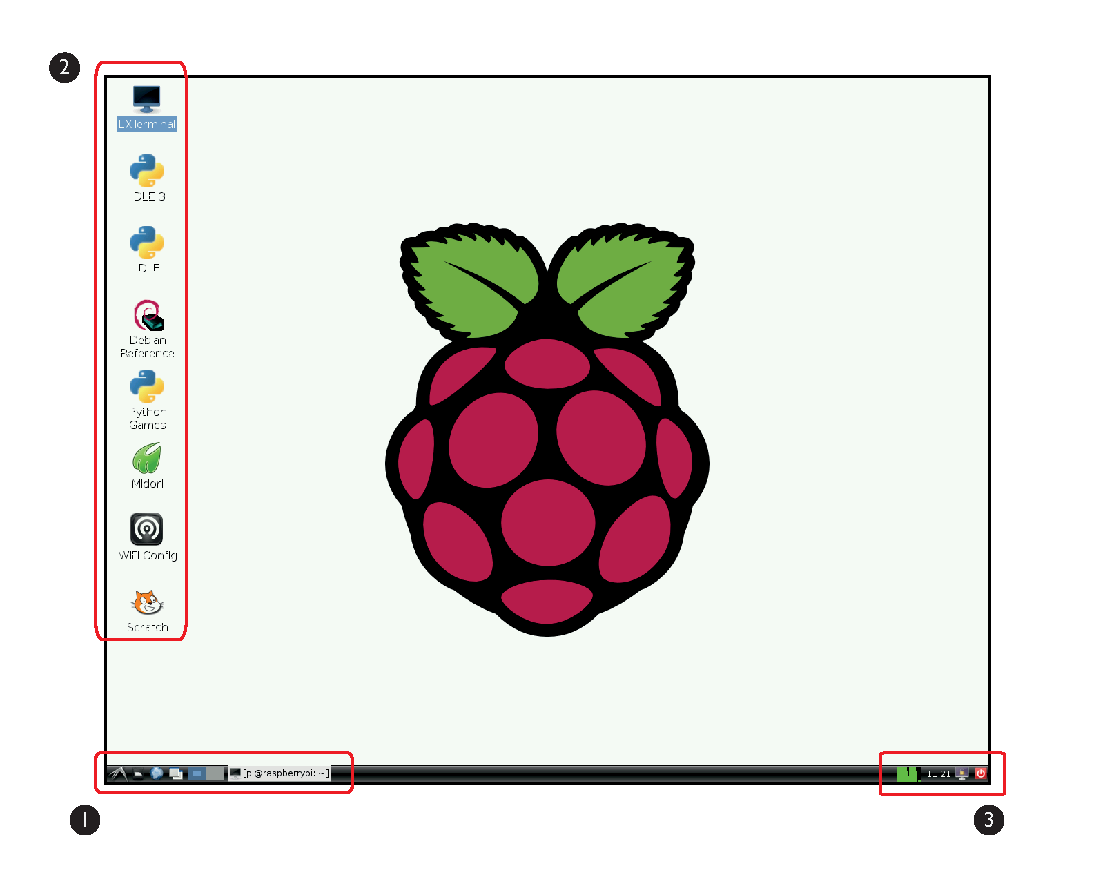
\includegraphics[width=14cm]{images/lxde-desktop}}
\caption{The Pi's default window manager is called LXDE.}\label{figure:lxde-desktop}
\end{figure}

\section{Configure mutt again using scp and ssh}

Once you've found your way around LXDE, fire up a terminal so that you can configure your Pi to read your University email using Mutt. Unlike the lab machines, the \cmnd{mutt}{mutt} command isn't installed by default on the Pi, so you'll need to do that yourself using:

\begin{ttoutenv}
\$ sudo apt-get install mutt
\end{ttoutenv}

Once the install has completed, you'll need to adjust Mutt's settings so that they once again point at your University email account. You could do this by following the instructions in the previous session's script again, but there's a much easier way: let's just copy the configuration file you created on the desktop PC last time, over to the Pi.

First you need to check that you still have the \fname{.muttrc} configuration file in your home filestore of your Computer Science account. You \textit{could} unplug all the cables from the Pi, connect them back into the desktop PC and check that way, but that's no fun (especially because we'd then have to reverse it all to do the next bit of the exercise). But you don't need to do that: you can check \concept{remotely}.

Find the hostname of the lab PC on your desk: there should be a sticker on both the PC itself and the monitor with a name such as \ttout{E-C07KILF3101}. If for some reason there isn't a sticker, Breakout~\ref{breakout:hostname} describes  several other ways to find a Unix machine's hostname.


\begin{linux}{Unix hostnames}
\label{breakout:hostname}
A machine's hostname identifies it on a network in a way that's usually a bit more human-readable than its IP address. There are various ways of finding out a machine's hostname:

\begin{itemize}
\item If you haven't logged into the PC and can see its screen, then it should be showing the hostname such as \ttout{E-C07KILF3101:} before the login prompt.
\item If you're already logged in to Unix, but have not started a window manager, your console prompt will be something like  \verb|[mrnoodle@E-C07KILF3101 ~]$| (where \ttout{mrnoodle} would be replaced by your own username, of course).
\item If you are logged in to the PC and inside a window manager, open a terminal window. It should show you the command line prompt, as above. You could also type \verb|echo $HOSTNAME|, or use the \cmnd{hostname}{hostname} command.
\end{itemize}
\end{linux}

Once you've got hold of the PC's hostname, you're going to use a \wikipedia{Secure_Shell}{Secure Shell} to connect to from the Pi to the the desktop, allowing you to type commands on the Pi that will be executed remotely via a shell that's running on the desktop PC. Open a terminal window on the Pi and issue this command:

\begin{ttoutenv}
\$ \cmnd{ssh}{ssh} [USERNAME]\!@\![HOSTNAME].cs.man.ac.uk
\end{ttoutenv}

replacing [USERNAME] with your University username, and [HOSTNAME] with the name of the PC in front of you. You'll need to enter your University password, and will most likely be presented with text something similar to this:

\begin{ttoutenv}
The authenticity of host 'E-C07KILF3101 (130.88.197.112)' can't be
established.
RSA key fingerprint is 20:6d:2d:90:5e:8f:9f:19:39:70:ce:48:a6:93:ec:4c.
Are you sure you want to continue connecting (yes/no)?
\end{ttoutenv}

Type \ttout{yes} (and hit enter) in response to the question. You should then be given a command prompt. You'll learn more about what this message actually means later in your programme, but for now just treat it as something that happens the first time you try to connect to a particular machine. Notice that this command prompt no longer says \ttout{pi@raspberrypi}, but rather has the name of the machine you've just remotely logged into. If your prompt still includes \texttt{pi@raspberrypi}, then something hasn't worked: you probably got the PC hostname wrong, or mistyped your University username or password, so just try again.

Type \cmnd{ls}{ls -a} to confirm that your \fname{.muttrc} file is still where you expect it to be, and if all is well then press \ctrl{d} to log out of the remote shell you just started, and you will return to the shell running locally on your Pi (you'll see the command prompt change back to being \texttt{pi@raspberrypi} again). Now we know that the file we want is there, we need to copy it from your Computer Science filestore onto your Pi's local filestore.

To do this, we're going to use the \cmnd{scp}{scp} (\concept{Secure Copy}) command, which in some ways behaves like \cmnd{cp}{cp}, but allows us to copy files \textit{between machines}.

Like \cmnd{cp}{cp}, the \cmnd{scp}{scp} command in its basic form takes two arguments, the first is the name of the source file (the one you want to copy), and the second is the name of the destination file (the one you want to create). The difference with \cmnd{scp}{scp} is that either (or less commonly, both) of these files can be on a remote machine, which means that you need to provide the command with enough information about the location of the remote file in terms of the hostname and file system, and any login details necessary to get at it. The syntax for providing this information is:

\begin{ttoutenv}
[USERNAME]\!@\![HOSTNAME]:[FILEPATH]
\end{ttoutenv}

So for example, if you wanted to retrieve a file called \fname{cheese.jpg} from the home directory of a user called \ttout{mrnoodle} that was stored on a machine with the hostname \ttout{mypc.example.com}, and you wanted the local copy of the file to be called \fname{mycheese.jpg} the command would be:

\begin{ttoutenv}
\$ scp mrnoodle@mypc.example.com:cheese.jpg mycheese.jpg
\end{ttoutenv}

Then, supposing you had edited the file \fname{mycheese.jpg} on your local machine and wanted to put the file back into the home directory of the \ttout{mrnoodle} account on the remote machine---but under a different name so as not to over-write the original---you would use the command:

\begin{ttoutenv}
\$ scp mycheese.jpg mrnoodle@mypc.example.com:newcheese.jpg
\end{ttoutenv}

We're not exactly sure why MrNoodle and cheese feature quite so prominently in this lab either, just go with the flow. To summarise the behaviour of \cmnd{scp}{scp}: if you prefix either or both of the source or destination files with the pattern \verb|[USERNAME]@[HOSTNAME]:| then you are referring to a file on a remote machine, otherwise you are referring to a local file in the same way that you would with a regular \cmnd{cp}{cp} command.

Now use your new-found knowledge of \cmnd{scp}{scp} to copy the \fname{.muttrc} file from your Computer Science account onto your Pi. You could use the hostname of the PC you're sitting at as the remote host, or alternatively you could use a server called \texttt{kilburn.cs.manchester.ac.uk} which is also set up to be able to see your Computer Science filestore. In fact, you could use the hostname of \textit{any} of the PCs in this lab, because your Computer Science filestore is accessible to them all---but it's probably antisocial to use a machine that someone else is sitting at, so for now stick to using the one in front of you, or \texttt{kilburn.cs.manchester.ac.uk}.



Conveniently, there's nothing in the \fname{.muttrc} file that is specific to the Computer Science account setup, so you can use it as-is for Mutt on the Pi (as usual, if you get stuck ask for help.)

Check that the file has copied over successfully using \cmnd{less}{less}, and then start up \cmnd{mutt}{mutt} from a terminal. If everything has gone to plan, you should now be able to read and compose emails on your Pi. You can of course install other mail clients if you want to; there is a slimmed-down version of Thunderbird for the Pi called Icedove (yes, yet another play on words), or a much leaner graphical client called Claws Mail (which, if you want to, can be installed using \ttout{sudo apt-get install claws-mail}). Remember, though, that the memory-card we've given you for your Pi is fairly small, so you probably don't want to clutter it up with unnecessary packages, and you should find that Mutt is perfectly okay for sending and reading the occasional email.

\subsection{Emailing your tutor}

To test that you've sucessfully set \cmnd{mutt}{mutt} up on the Pi, use it to send a friendly email to your tutor to tell him or her that you'vbe reached this point of the lab . If you've not figured out your tutor's email address yet, you can find it using Epiphany at \\
\url{http://www.cs.manchester.ac.uk/about-us/staff/}

\section{X Windows again}

As we mentioned before, the X Windows system is a powerful system, and although it was designed a long time ago (around 1984), it was in many ways way ahead of its time (rather like the design of Unix itself.)

Remember that the GUI you're now using on the Pi consists of two systems working together: X Windows (which amongst other things gives software access to the display hardware), and the Window Manager / Desktop environment (in this case, LXDE) that provides the WIMP-style features such as movable windows and clickable controls. The X Windows system operates as a \concept{Client/Server architecture}, where the server part does the drawing of stuff onto the screen, and clients request that things be drawn. One of the really nice features of X Windows is that it doesn't care too much about where the requests to draw things come from. Typically they come from processes that are running on the same computer as the X Server, but this need not be the case as you're about to demonstrate.

Log back in to the lab PC using the \cmnd{ssh}{ssh} command, but this time include a \texttt{-X} switch before your username, like:

\begin{ttoutenv}
\$ ssh -X [USERNAME]\!@\![HOSTNAME]
\end{ttoutenv}

The \ttout{-X} switch (note that it's an uppercase X) tells the \cmnd{ssh}{ssh} program to send any graphics instructions generated on the remote system back through the network to the X Server running on the local machine.

Confirm that you are indeed logged into your Computer Science account by checking the command prompt and using \cmnd{ls}{ls} to make sure the files in your home directory are the ones you'd expect (or use one of the techniques described in Breakout~\ref{breakout:hostname} to check the hostname), and then type:

\begin{ttoutenv}
\$ xeyes
\end{ttoutenv}

\wikipedia{Googly_eyes}{Googly eyes} that follow the mouse! What's not to like? Well, okay, perhaps not hugely exciting in itself, but what's actually happening here is rather interesting and quite sophisticated. The \cmnd{xeyes}{xeyes} program is running on the remote machine (the desktop PC); but the instructions to draw its graphical output are being forwarded over the secure shell connection you've made from the Pi to the remote machine, so that the Pi's X Windows system receives them. Make sure that the terminal window you used to start \cmnd{xeyes}{xeyes} is the active window, then press \ctrl{c} to quit \cmnd{xeyes}{xeyes}, and instead try running \cmnd{xterm}{xterm}. You should see a new terminal window appear on your Pi's screen (which probably looks slightly different to the terminal you launched on the Pi a moment ago; it does essentially the same thing though). This X Terminal, rather like \cmnd{xeyes}{xeyes}, is actually running on the desktop machine---only its graphical representation is appearing on your Pi (if you use \cmnd{ls}{ls} in that terminal, you'll see that its your Computer Science account that's visible, rather than your Pi's filestore and you can confirm this another way using the \cmnd{hostname}{hostname} command). Look at Figures \ref{figure:x-on-pi} and \ref{figure:x-via-ssh} for a diagrammatic representation of what's just happened. Now exit this X Terminal by typing \ctrl{d} in it.

\begin{figure}
\centerline{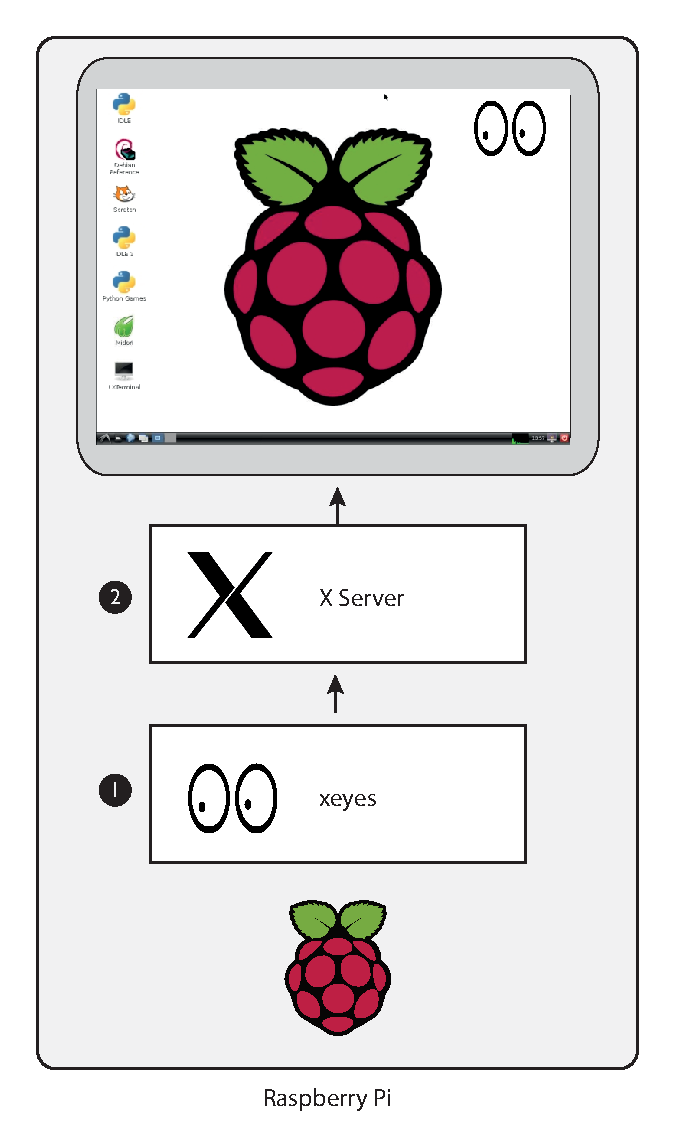
\includegraphics[width=8cm]{images/x-on-pi}}
\caption{In Unix, when you run a program such as \cmnd{xeyes}{xeyes} on your local machine, it doesn't draw directly to the screen, but instead communicates with an X Server that by default is running on the same machine. In our example, the xeyes program \protect\circled{1} connects to its local X Server \protect\circled{2}, and asks it to draw a window containing two ellipses to represent eyeballs, and then does some calculations to work out where to draw the two smaller ellipses to represent the pupils of the googly eyes so that they follow the mouse pointer. The X Server then communicates with the graphics hardware of the local machine in order to make things appear on the display that you see as a user. }\label{figure:x-on-pi}
\end{figure}

\begin{figure}
\centerline{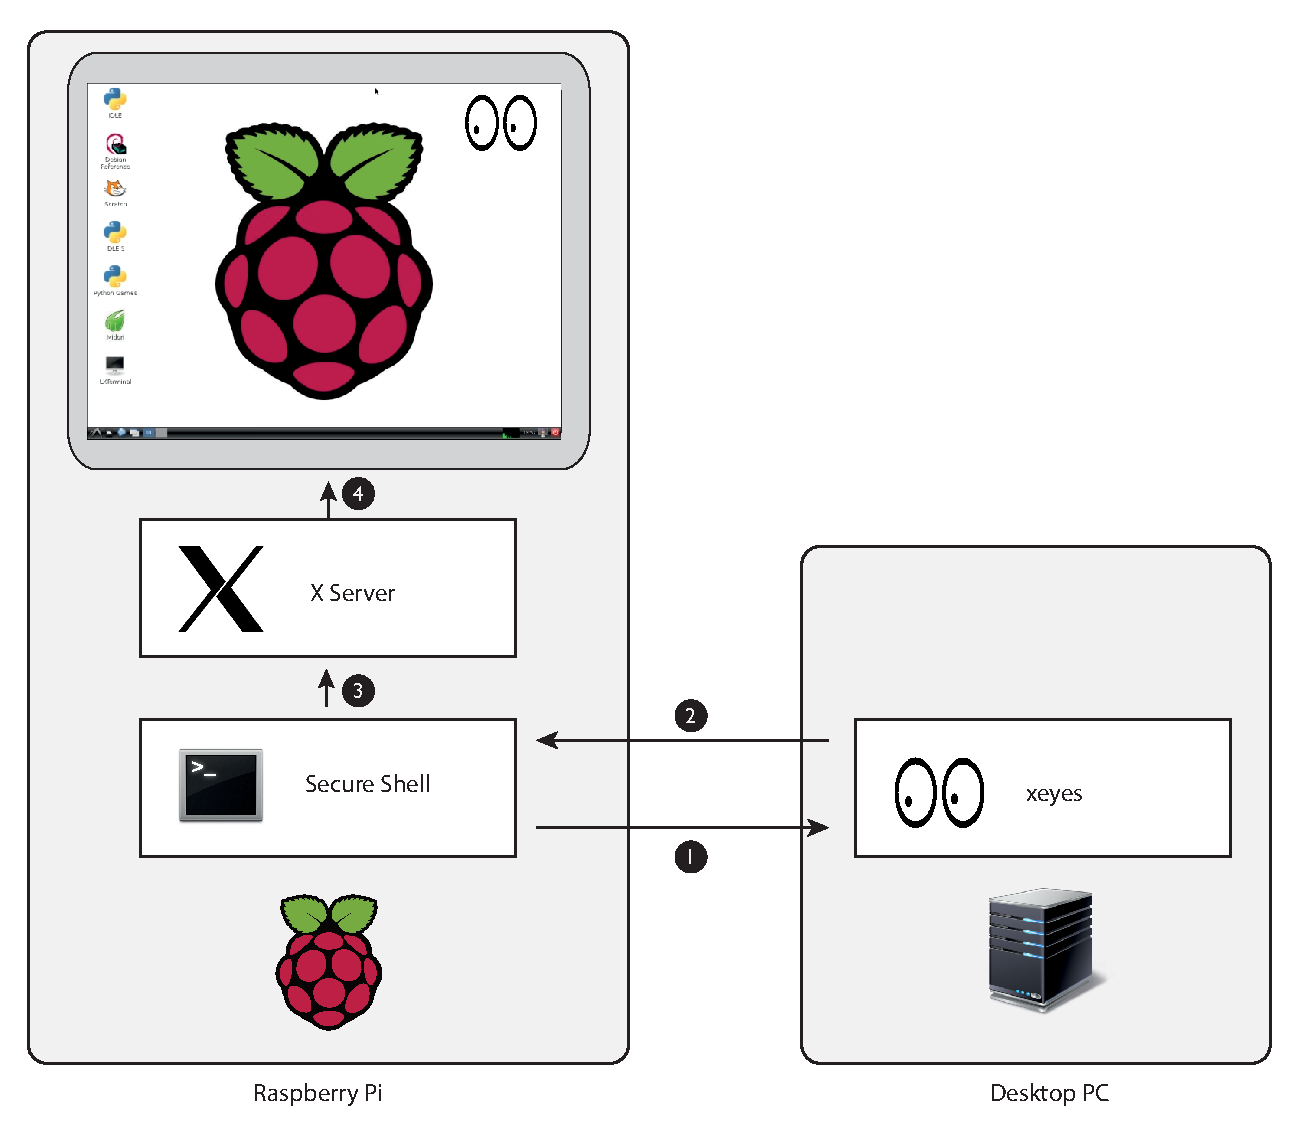
\includegraphics[width=17cm]{images/x-via-ssh}}
\caption{One of the powerful features of the X Windows system is that the program generating graphical output, and the display on which the graphical output appears need not be on the same physical machine. In this example, we've used a Secure Shell connection from the Pi \protect\circled{1} to make a connection to the desktop PC, and have used the \ttout{-X} option to ask that any graphical instructions for the X Windows system get routed back through that connection. We then start the xeyes program on the desktop PC. Now although the calculations to draw the googly eyes are being done on the remote PC, the instructions to draw ellipses are sent back via the \cmnd{ssh}{ssh} connection to the Pi  \protect\circled{2}, and are \protect\circled{3} routed to the X Server that's running on the Pi. As before, the X Server \protect\circled{4} interprets these instructions (not caring that they originated on another machine), and draws the eyes on the display that's physically connected to the Pi.}\label{figure:x-via-ssh}
\end{figure}



%How could you use this feature to your advantage to give you a temporary graphical mail client (or perhaps to use Firefox as a web browser, rather than Epiphany) on the Pi without needing to install any packages on the Pi itself?


\section{A Simple Web Server}

This next exercise involves setting up a simple web server on the Pi, but before we can do that you'll need to create some basic web pages to display.

Start up a terminal on your pi, and use the \cmnd{mkdir}{mkdir} to create a directory called \fname{htmlexample1} in your home directory, and in that directory, use \ttout{nano} to create a file called \fname{index.html} with the following content:

\begin{ttoutenv}
<html>
  <body>
    Hello world!
  </body>
</html>
\end{ttoutenv}

From within that directory, run the command:

\begin{ttoutenv}
\$ \cmnd{python}{python} -m SimpleHTTPServer
\end{ttoutenv}

which starts a very basic \concept{Web Server} and then use Epiphany to browse to the following URL:

\begin{ttoutenv}
http://localhost:8000
\end{ttoutenv}

If your browser displays a page saying `Hello World', pat yourself on the back---you've just created a web page \textit{and} set up a simple web server to host it. The URL you used to view this page may look a bit odd compared with others you have seen. The \texttt{http://} part you'll no-doubt be familiar with from other web-addresses that you've seen; the \texttt{localhost} part is a convention that means `this machine'. The section of the URL that follows \texttt{localhost} may be even less familiar: this is the \textit{port} (for now just think of this as a kind of communication channel) on which the simple web-server that you've set up is serving web pages; by default web browsers expect servers to use port 80, but the \ttout{python -m SimpleHTTPServer} command you used here defaults to port 8000, so we had to add that to the URL. We'll leave the issue of ports there for now, and revisit that in more detail in the 2nd semester in \courseunit{COMP18112}.

\subsection{A slightly more interesting web page}

Next you're going to create a slightly more interesting web page that contains a paragraph describing who you are, which programme you're on (e.g. Computer Science, Software Engineering, etc.), and which contains a picture of yourself as well as the image you created in the previous session using Inkscape.

Use \cmnd{cd}{cd} to change to your home directory, and then \ttout{curl} to fetch a gzipped tar of the example Mr Noodle web page that we've created for you from:
\\

{\small

\url{http://studentnet.cs.manchester.ac.uk/ugt/COMP10120/files/mrnoodle.tar.gz}
}
\\

In your home directory, use \cmnd{tar}{tar} to `untar' this bundle of files using the command:

\begin{ttoutenv}
tar xvzf mrnoodle.tar.gz
\end{ttoutenv}

Notice that this time we've added an extra \texttt{z} switch to the \cmnd{tar}{tar} command's argument which tells tar to both `unzip' and then `untar' the file in one go (if you remember when you downloaded the Quake bundle in the first Pi session, you did this in two stages, first using \cmnd{gunzip}{gunzip}, and then \cmnd{tar}{tar}).

You should end up with a \fname{htmlexample2} directory containing an \fname{index.html} file and two image files, one in \fname{.png} and the other in \texttt{.jpg} format.

Use a text editor to change the content of \fname{index.html} so that it says something about you. Don't worry about finely crafted words here---this is really just a way of creating some files that we can get you to edit in various ways a little later on. A few sentences will do, and you can always change it later. Replace the default images we've provided with something that's relevant to you. Perhaps a photograph of yourself, and whatever it was you drew in Inkscape would work here (though note, you'll have to reopen the picture in Inkscape and export it to a bitmap format such as \texttt{.jpg} or \texttt{.png} to be able to include it in your webpage).

You've already learned several ways of getting files onto your Pi, but here's a reminder:
\begin{itemize}
\item You could mail the photo to yourself, and use Mutt to save the attachment onto the Pi (for help on how to do this see Mutt's online FAQ at \url{http://dev.mutt.org/trac/wiki/MuttFaq})
\item If the picture is already on the web somewhere, you could use Epiphany to find and save it.
\item Alternatively for images on the web, you could use \ttout{curl} to fetch it directly from a URL to a file.
\item You could use \ttout{scp} to copy it from some other machine directly to your Pi.
\item Or if all else fails, you could use a USB device to copy it from one place to another.
\end{itemize}

If you need more guidance on how to write the web page itself there are plenty of tutorials on the web (search for something like `basic HTML tutorial').

To finish this section, start up the SimpleHTTPServer that we used earlier \textit{but this time in your htmlexample2} directory, and use Epiphany to check that your web page is displaying correctly.

\FloatBarrier

\section{Headless Pi}
\label{section:headless}

\begin{stdframe}{light-gray}%
  \centerline{\textbf{Don't Panic!}}
The rest of this lab session exposes you a fair number of quite advanced concepts pretty quickly, and we don't expect all of them to sink in this first time round. Stay calm.  Don't panic. Just follow our instructions and everything will be fine; if you get lost or things aren't going to plan, just ask a member of lab staff to help you get back on track, and we'll revisit these ideas in later labs where there will be more opportunities to put them into practice and make sure everything makes sense.
\end{stdframe}

The Pi can be used as a respectable desktop machine, but it really comes into its own as a \concept{server} or controller for other pieces of hardware. In this section we'll use the Pi in what is called `headless' mode---that is without its own screen and keyboard---to create a proper web server to host your pages.

In a terminal, type the command \ttout{ifconfig}, short for `interface configuration', which will give you details about the network configuration on the Pi. This will return something along the lines of

\begin{ttoutenv}
eth0      Link encap:Ethernet  HWaddr b8:27:eb:a5:d5:82
          inet addr:10.2.233.1  Bcast:10.2.239.255  Mask:255.255.248.0
          UP BROADCAST RUNNING MULTICAST  MTU:1500  Metric:1
          RX packets:39778 errors:0 dropped:0 overruns:0 frame:0
          TX packets:4338 errors:0 dropped:0 overruns:0 carrier:0
          collisions:0 txqueuelen:1000
          RX bytes:18251497 (17.4 MiB)  TX bytes:651537 (636.2 KiB)

lo        Link encap:Local Loopback
          inet addr:127.0.0.1  Mask:255.0.0.0
          UP LOOPBACK RUNNING  MTU:16436  Metric:1
          RX packets:105 errors:0 dropped:0 overruns:0 frame:0
          TX packets:105 errors:0 dropped:0 overruns:0 carrier:0
          collisions:0 txqueuelen:0
          RX bytes:8550 (8.3 KiB)  TX bytes:8550 (8.3 KiB)
\end{ttoutenv}

This tells you that the Pi has two network devices currently active: one called `eth0', which represents the physical ethernet socket into which you plugged the blue network cable, and which allows the Pi to communicate with other computers on the network (and in this case, on the internet); and a second one called `lo' which is a `virtual connection' or \concept{local loopback} connection that allows the Pi to route network traffic back to itself (this is how the `localhost' trick you used earlier to look at web pages on the Pi worked). You can learn a lot more about network configuration in the second year Computer Networks course (\courseunit{COMP28411}).

The thing we're interested in right now is the IP Address that's been allocated to your Pi. Look for the line in the \texttt{eth0} block of text that says \texttt{inet addr:} and note down the number that follows this in your logbook (in the case of our example that is \texttt{10.2.233.1} but in your case it will probably be something else). Don't worry too much about what this number means or where it came from for now---we'll return to this in \courseunit{COMP18112} in the second semester. For now, just treat this as being a unique number that identifies your Pi on the Computer Science network.

Quit the graphical environment, and log out of your Pi by typing \cmnd{logout}{logout} at the console's command prompt (or you can press \ctrl{d} to achieve the same effect). Leave the network connection and power supply plugged in, but disconnect the mouse/keyboard lead, and reconnect them to the desktop PC. Switch the monitor over to display the desktop PC's screen, and log in to that with your University credentials.

Once you're in the graphical window environment on the desktop PC, start up a terminal, and use \cmnd{ssh}{ssh} to log into your Pi:

\begin{ttoutenv}
\$ ssh pi@[IPADDRESSOFPI]
\end{ttoutenv}

replacing [IPADDRESSOFPI] with the IP Address you noted down a moment ago. Since this is the first time you're logging in from your CS account to your Pi, expect to see the `The authenticity of host' warning again; just say `yes' to the prompt, and enter your Pi user's password.

Change directory to the \fname{htmlexample1} directory you created for your web-page earlier, and re-start the simple Python web server.

Next, start up Firefox on your desktop using the keyboard shortcut you created in the previous lab session, and enter the URL:

\begin{ttoutenv}
http://[IPADDRESSOFPI]:8000
\end{ttoutenv}

and you should see your web page appear, served off your Pi to the desktop machine just like a real web server. Get the person next to you to see if they can see your web page from their machine by using your Pi's address; and return the favour by checking that theirs is also working (it's worth noting that the IP addresses of the Pis are only visible within the School of Computer Science, so pages served off your Pi will not be visible on the wider Internet).


\subsection{Setting up Apache, a proper web server}

The simple Python-based web server that you've been running so far is doing the bare minimum necessary to allow HTML pages to be fetched by a browser. Although it was a handy way of getting you going with web server technology, it's a long way off being the kind of fully-featured web server you would need to run a modern website. Fortunately, the Apache HTTP Server---the software that \textit{is} used to run over half the world's websites---is Open Source and runs quite happily on a Raspberry Pi. You wouldn't want to be powering the next eBay or Facebook from a Pi, but to illustrate the principles, it'll do the job nicely.

Before we install Apache on your Pi, there's a bit of housekeeping to do that will conveniently expose you to a few more Unix concepts that we've rather skated over so far.

\subsection{Permissions, users and groups}

Right at the beginning of these sessions you logged in to the Pi as a particular user called `pi', and on the desktop machines you've been logging in using your University username and password. It's fairly obvious what the general principles are here---logging in with a username and password is a way of protecting `your stuff' from being seen or messed around with by other users. Roughly speaking this means two things: first, and most obviously, files created by you should be in some sense `owned' by you so that you can control who can see/modify them; second, and perhaps less obviously, processes that you start---whether from the command line or the graphical environment---are also `yours' and have certain privileges/restrictions that are associated with your user.

For this to work, it means that both the Unix file system and its way of dealing with processes need to be aware of the notion of a user. Back in the terminal that's connected by \cmnd{ssh}{ssh} to your Pi, use \cmnd{cd}{cd} to change to your home directory and type \cmnd{ls}{ls -l} to list the files there in what's called `long format' (the \ttout{-l} switch means `give me extra information about each file'). You'll see something like Figure~\ref{figure:longformls} (but without the coloured background, which we've added to help distinguish the different columns in the figure).

\begin{figure}
\centerline{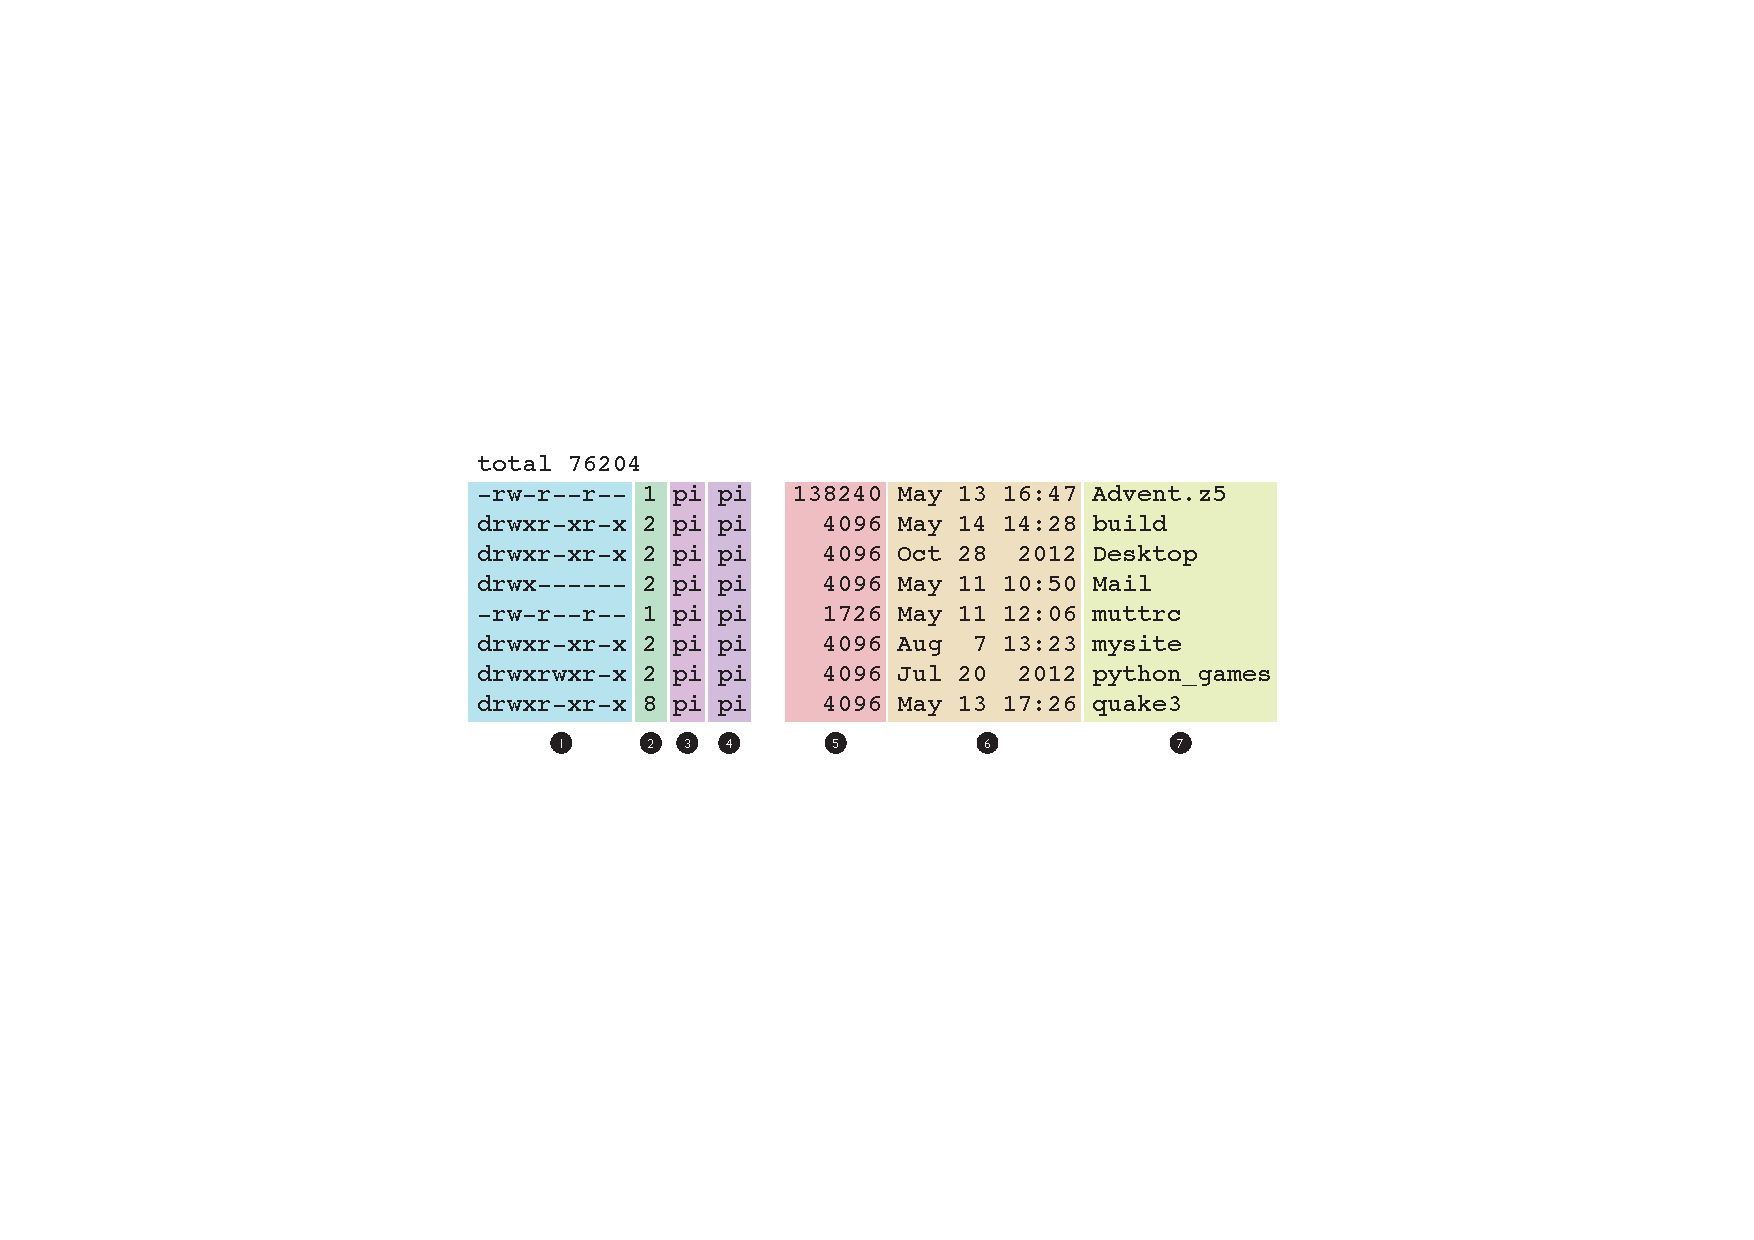
\includegraphics[width=14cm]{images/longformls}}
\caption{An example of the `long format' output from ls.}\label{figure:longformls}
\end{figure}

Working from right to left in Figure \ref{figure:longformls}, column \protect\circled{7} contains the filename, column \protect\circled{6} gives the date that the file was last modified (the exact format of the date will vary so as to always be `useful'; older files will have a year instead of an exact time, for example) and column \protect\circled{5} shows the size of the file in bytes. Columns \protect\circled{4} and \protect\circled{3} give the group and user to which the file belongs; we'll come back to this in a moment. Column \protect\circled{2} shows the number of links associated with the file (ignore this for now), and finally column \protect\circled{1} gives a summary of the file's permissions, which we'll look at again shortly.

In our example, the file's user (Column \protect\circled{3}) is not surprisingly `pi', which is the username under which you logged in. Run

\begin{ttoutenv}
\$ ls -l /
\end{ttoutenv}

(i.e. `long format list of the root directory), and you'll see that the files at the top of the filesystem are owned by a user called \ttout{root}.

As well as being owned by a particular user, each file is associated with a \concept{group} (shown in column \protect\circled{4}, which in this case is a group called `pi' too; although both the user and the group are called pi here, they are different things). Every user is a member of one or more groups. The idea of a Unix group is quite straightforward: it's a mechanism to allow collections of users to share resources with one another in a controlled way, while stopping other unwanted users from being able to access those resources. For example, you might want to say ``Only I as this file's creator am allowed to modify or delete this file, but other members of my Tutorial Group can read the file's content, and the file is inaccessible to everybody else''. In Unix each file can have three different types of access permission: read, write and execute (run). These permissions can be set for three different categories of user: user (`owner'), group (a specific set of users) and `other' (which means `everyone else').

The file permissions shown in column \protect\circled{1} of Figure \ref{figure:longformls} consist of 10 `slots' as shown in more detail in Figure \ref{figure:fileperms}. The first slot indicates the type of the file, and appears as a \ttout{-} for a regular file or a \ttout{d} for a directory. The next three slots represent the \concept{user}'s  permissions and can consist of any combination of \ttout{r} for `readable', \ttout{w} for writable and \ttout{x} for executable. The next three slots show the read/write/execute permissions for members of the file's \concept{group}, and the last three slots show the same set of available permissions for \concept{other} (i.e. anyone else with access to the system). Execute permissions when applied to a directory mean that particular set of users can access the directory's contents.

\begin{figure}
\centerline{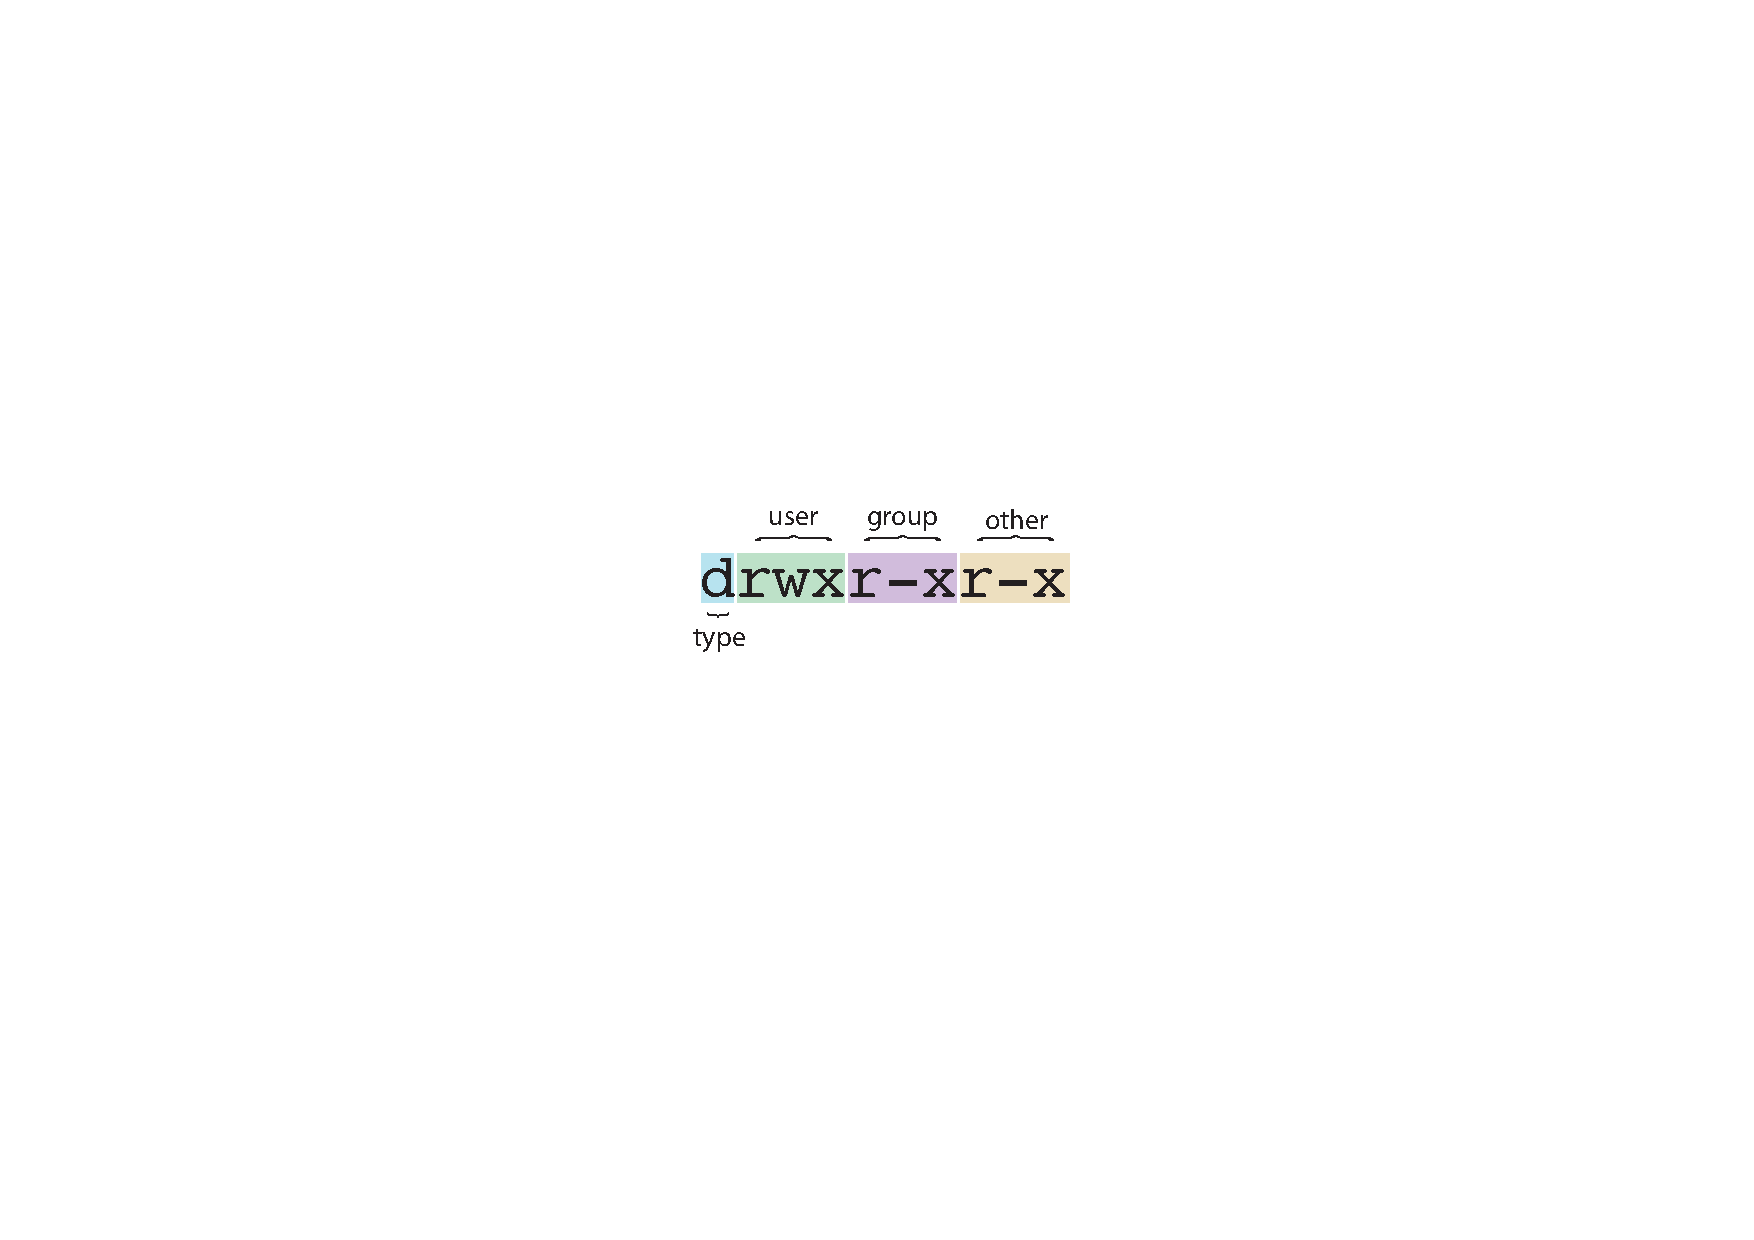
\includegraphics[width=7cm]{images/filepermissions}}
\caption{Unix file permissions as shown with \ttout{ls -l}. In this example shows the permissions for a directory that can be read from, written to and listed by its user (owner), but only read and accesed by group members or anyone else.}\label{figure:fileperms}
\end{figure}

We'll come back to file permissions in more detail shortly. In the meantime, let's look at the ownership model for processes. Type:

\begin{ttoutenv}
\$ ps waux
\end{ttoutenv}
% $

to list any processes that are currently running (you'll probably need to widen the terminal window to see the output properly). The \cmnd{ps}{ps} command is unusual in that if used with no arguments, its output is largely uninformative. It's also unusual in that explaining what even the most basic arguments do and how they interact (i.e. the \ttout{waux} options in this case), is quite complex---so for now just treat this as a special recipe that does something useful. Note that there's no hyphen in front of the options in this case.

Look at the rightmost column of the output (which has the heading `COMMAND') and you should see a few familiar process names such as \cmnd{bash}{bash}, \ttout{startx}, and the \cmnd{ps}{ps} process itself in amongst many commands that will be unfamiliar to you at the moment. The leftmost column tells you who owns the processes, and you'll see that some of them are owned by you (or, rather by the user `pi'), and others are owned by the root user. Most of the processes that you're seeing have been started as part of the window manager system, or are in one way or another associated with X Windows; the rest are `housekeeping' processes the details of which we don't care about for now.

If you think back to what you learned about the hierarchical relationship between processes in the first Pi lab, it should be starting to become clear how the `family tree' of processes when combined with the notion of users and resource ownership knit together nicely to give a secure multi-user system. When you first log in to a Unix machine, a single process is started on your user's behalf (in most cases this is a command shell). From that shell you can start other processes, which could be individual commands like \ttout{tar} or \ttout{ls}, or could be a whole window manager system such as GNOME or LXDE; in either case though, these inherit the properties of the parent shell in terms of being owned by the same user. Then, any processes that are started by the window manager also inherit the same user properties, and so forth.

\subsection{Back to that webserver}

Anyway, let's get back to setting up the Apache web server. When you ran the Python web server, that was a process owned by you, and because we didn't do anything special to protect it, if you closed the shell/terminal that was used to start it, it too would die. Generally speaking, you'd want a web server to continue running whether anyone was logged into the machine or not, so this isn't ideal. The other issue with starting a web server in this way is that because the process is owned by you, it has access to all your files---so if a malicious hacker was able to take control of the web server process, he or she would be able to read or even delete your work, which clearly isn't a good thing.

So to set up a web server properly we need to

\begin{itemize}
\item make sure that it can continue to function after you've logged out, and
\item somehow make sure that it can only access a specific set of resources that represent the website, and not run riot around your filestore doing bad things.
\end{itemize}

Let's first tackle the issue of a shared directory; this is quite easy to set up using Unix's group mechanism.

By default, the Apache package that we're going to install shortly is set up to serve web pages from a directory called \fname{/var/www} and although you can change it in Apache's configuration files to be elsewhere, that's as good a place as any for what we need.

Let's go ahead and install Apache using the command:

\begin{ttoutenv}
\$ sudo apt-get install apache2
\end{ttoutenv}

It's a reasonably large package so may take a little while to install; just be patient. Once that's completed, take a look in \fname{/var} using \ttout{ls -l} and you should see a directory in there called \fname{www} which is owned by root.

Before we start serving any web pages, there are a few security issues that we need to take into account. In its simplest form, where you're just serving static web pages (i.e. HTML files), Apache is secure enough, but as soon as you start creating web sites where users can add and modify content on your server, you potentially open yourself up to malicious damage, so it's best to take some initial precautions.

Take a look at the permissions for \fname{/var/www}, which was created when you installed the Apache package, and you will see that they are set to \ttout{drwxr-xr-x} which means `this is a directory that the owner can read, write and access the contents of, and which both group and other users can only read and access'. Notice too that there's a single file in that directory called \fname{index.html}, which is an `it works!' declaration that you can use to test that Apache is doing the right thing (and which we'll do shortly). The important thing here is that anybody or any process that is not running as the root user has only got \concept{read} and \textbf{not} \concept{write} access to the contents of the \fname{/var/www} directory structure---and this is exactly what we want. They can look, but not touch, and so can't break anything.

But how do we get content into the \fname{/var/www} directory so that it can be served by Apache? We could simply use \fname{sudo} to give ourselves root privilege every time we need to modify a file, but that's a rather clumsy solution: we may not want other users on our machine to have root access at all, and in any case you really do want to keep sudo commands to a minimum so that you don't accidentally do something bad to your system. So let's create a new group that will represent users on the Pi that are allowed to put content into that directory. Use the command \cmnd{addgroup}{addgroup} to create a new group called \ttout{www-contrib} (for `web contributors'). The syntax is straightforward:

\begin{ttoutenv}
\$ sudo addgroup www-contrib
\end{ttoutenv}

And you should see that a new group has been created with a Group Identifier (GID) probably set to 1004.

Change the group ownership of \fname{/var/www} to be \ttout{www-contrib} using the command

\begin{ttoutenv}
\$ sudo chgrp -R www-contrib /var/www
\end{ttoutenv}

and check that this has changed using \ttout{ls -l}. Note that we're using the \ttout{-R} option to \cmnd{chgrp}{chgrp}, which means `apply this change not only to /var/www itself, but to all files and directories contained within it' (\ttout{R} here stands for \wikipedia{Recursion}{recursive}). Next we need to add the pi user to that group. Type

\begin{ttoutenv}
\$ groups
\end{ttoutenv}

to see what groups your user is already a member of (you'll see things like \ttout{pi}, \ttout{adm}, \ttout{dialout}, \ttout{cdrom}, \ttout{sudo} and several others). Use the command

\begin{ttoutenv}
\$ sudo usermod -a -G www-contrib pi
\end{ttoutenv}

to add the Pi user to the www-contrib group. The \ttout{usermod} command can be used to modify lots of things about a user; here we are using with the combination of \ttout{-a} and \ttout{-G} to mean `append this group to the user's list of groups'. You'll need to log out and back in again to see this change take effect, so do that now and then run the \ttout{groups} command to confirm that \ttout{pi} is now indeed a member of group \ttout{www-contrib} as well as the other original groups.

% \begin{diversion}{About groups}
% \label{diversion:aboutgroups}
% Explain what the other groups are for
% \end{diversion}

We now need to make the \fname{/var/www} folder \concept{writable} by members of our new group, so do that using the command

\begin{ttoutenv}
\$ sudo chmod -R g+w /var/www
\end{ttoutenv}

which reads as `modify the permissions of the directory /var/www and any files/directories in it to add write access for members of its group'.

Now if all has gone to plan, the user pi should be able to read and write to the directory \fname{/var/www}. Try this out by editing the content of the \fname{index.html} file that's in that directory (and which was created when you installed Apache) to say something different from the default text.

We're finally ready to start Apache. Use the Apache Control command

\begin{ttoutenv}
\$ sudo apachectl start
\end{ttoutenv}

to initialise the server (you can use a similar command with \texttt{stop} to shut it down again), and then use \cmnd{ps}{ps waux} to confirm that you can see several processes with \texttt{apache} in the name now running. Note that although you started the server with \cmnd{sudo}{sudo} which runs things as root, that the owner of the apache processes is \fname{www-data}. The \ttout{apachectl} command has restricted apache to running as a regular, non-root user, and you should by now be able to work out why having a web server running as root would be a Bad Thing from a security point of view.

On the desktop machine use a web browser to see what content the Pi is now serving. The URL will be

\begin{ttoutenv}
http://[IPADDRESSOFPI]
\end{ttoutenv}

and since we're now using a standard web server on a standard port (port 80), there's no need to add the :8000 port number as we did in Section \ref{section:headless}.

You should see the `It works!' page appear, with whatever modification you made to it a moment ago.

Nearly finished. Copy the content from your \fname{htmlexample2} directory so that its served via Apache, and check using a web browser that the `It works!' page has been replaced by your own masterpiece.

\section{Shutting down gracefully}

That's all the exercises done for this lab session; but before you finish  there's one last important thing to do. Make sure you use the \cmnd{halt}{halt} command to shut your Pi down cleanly, otherwise you risk losing some of your work by corrupting its file system. You can do this over a \cmnd{ssh}{ssh} connection quite safely, so you don't need to reconnect the keyboard/mouse/monitor to the Pi, just type \texttt{sudo} \cmnd{halt}{halt} in the secure shell that's running on the Pi. Of course, you shouldn't be surprised when secure shell gets disconnected as the Pi begins to shut itself down.

\section{Finishing up}
Don't worry if not everything you've done in this session has sunk in yet---you've encountered a lot of new concepts in this session, and we'll be revisiting everything in one form or another in future labs. This is the last lab that uses your Pi for a while now, and in the next session we'll be introducing you to the virtual learning environment that will be used for several of the course units this year, and giving you an opportunity to practise some of the skills and techniques that we've covered already. But this isn't the last you'll see of the Pi---you'll be using it as part of your group project in \courseunit{COMP10120}, so please don't lose it. In the meantime, remember that even if you do something wrong on the Pi, it's very easy to restore it back to a clean state, and we encourage you to explore Unix and have fun with this fantastic bit of hardware.
